% Objectives / Challenges
% SE-PIM Architecture --> Hardware Stuff
% -- Remote attestation and Secure channel (Short)
% -- Hardware acceleration for encrypted data flow
% -- Preventing side-channels during computation
%    -- Controlled access channel
%    -- DRAM lockdown 
%       -- gives PIM core control over DRAM access control
% -- 
% Programming Model
% -- 
% Implemenation 
% Evaluation
% Discussion
% Related Work
% Conclusion




\section{SE-PIM Architecture}
\label{sec:design}
The design of \thename specifically mitigates the challenges explained in the previous section. Our design brings imperative changes for \baseline to overcome the unique challenges in achieving its objectives. We explain each architectural change and how they mitigate the challenges in this section. 


% \cref{subsec:hardware} illustrates the overview of \thename architecture.  We explain remote attestation and secure channel establishment in \cref{subsec:attestation}. \cref{subsec:aes-dma} illustrates our design for encrypted data flow acceleration, addressing \challenge{1}. \cref{subsec:side-channels} elaborates how we address the challenges \challenge{2}, \challenge{3} and \challenge{4} with the introduction of DRAM lockdown and the controlled access channel.


% In \cref{subsec:access-control}, we describe the DRAM lockdown logic, which addresses \challenge{3} and \challenge{4} . Our secure memory access interface in \cref{subsec:secure-access} allows the host enclave to hide its memory access pattern, which solves \challenge{2}. Finally, to deal with \challenge{1}, we introduce AES acceleration to the DMA engine to efficiently transfer encrypted data between PIM local memory and the memory bank (\cref{subsec:aes-dma}).


\begin{figure}[t]
    \centering
    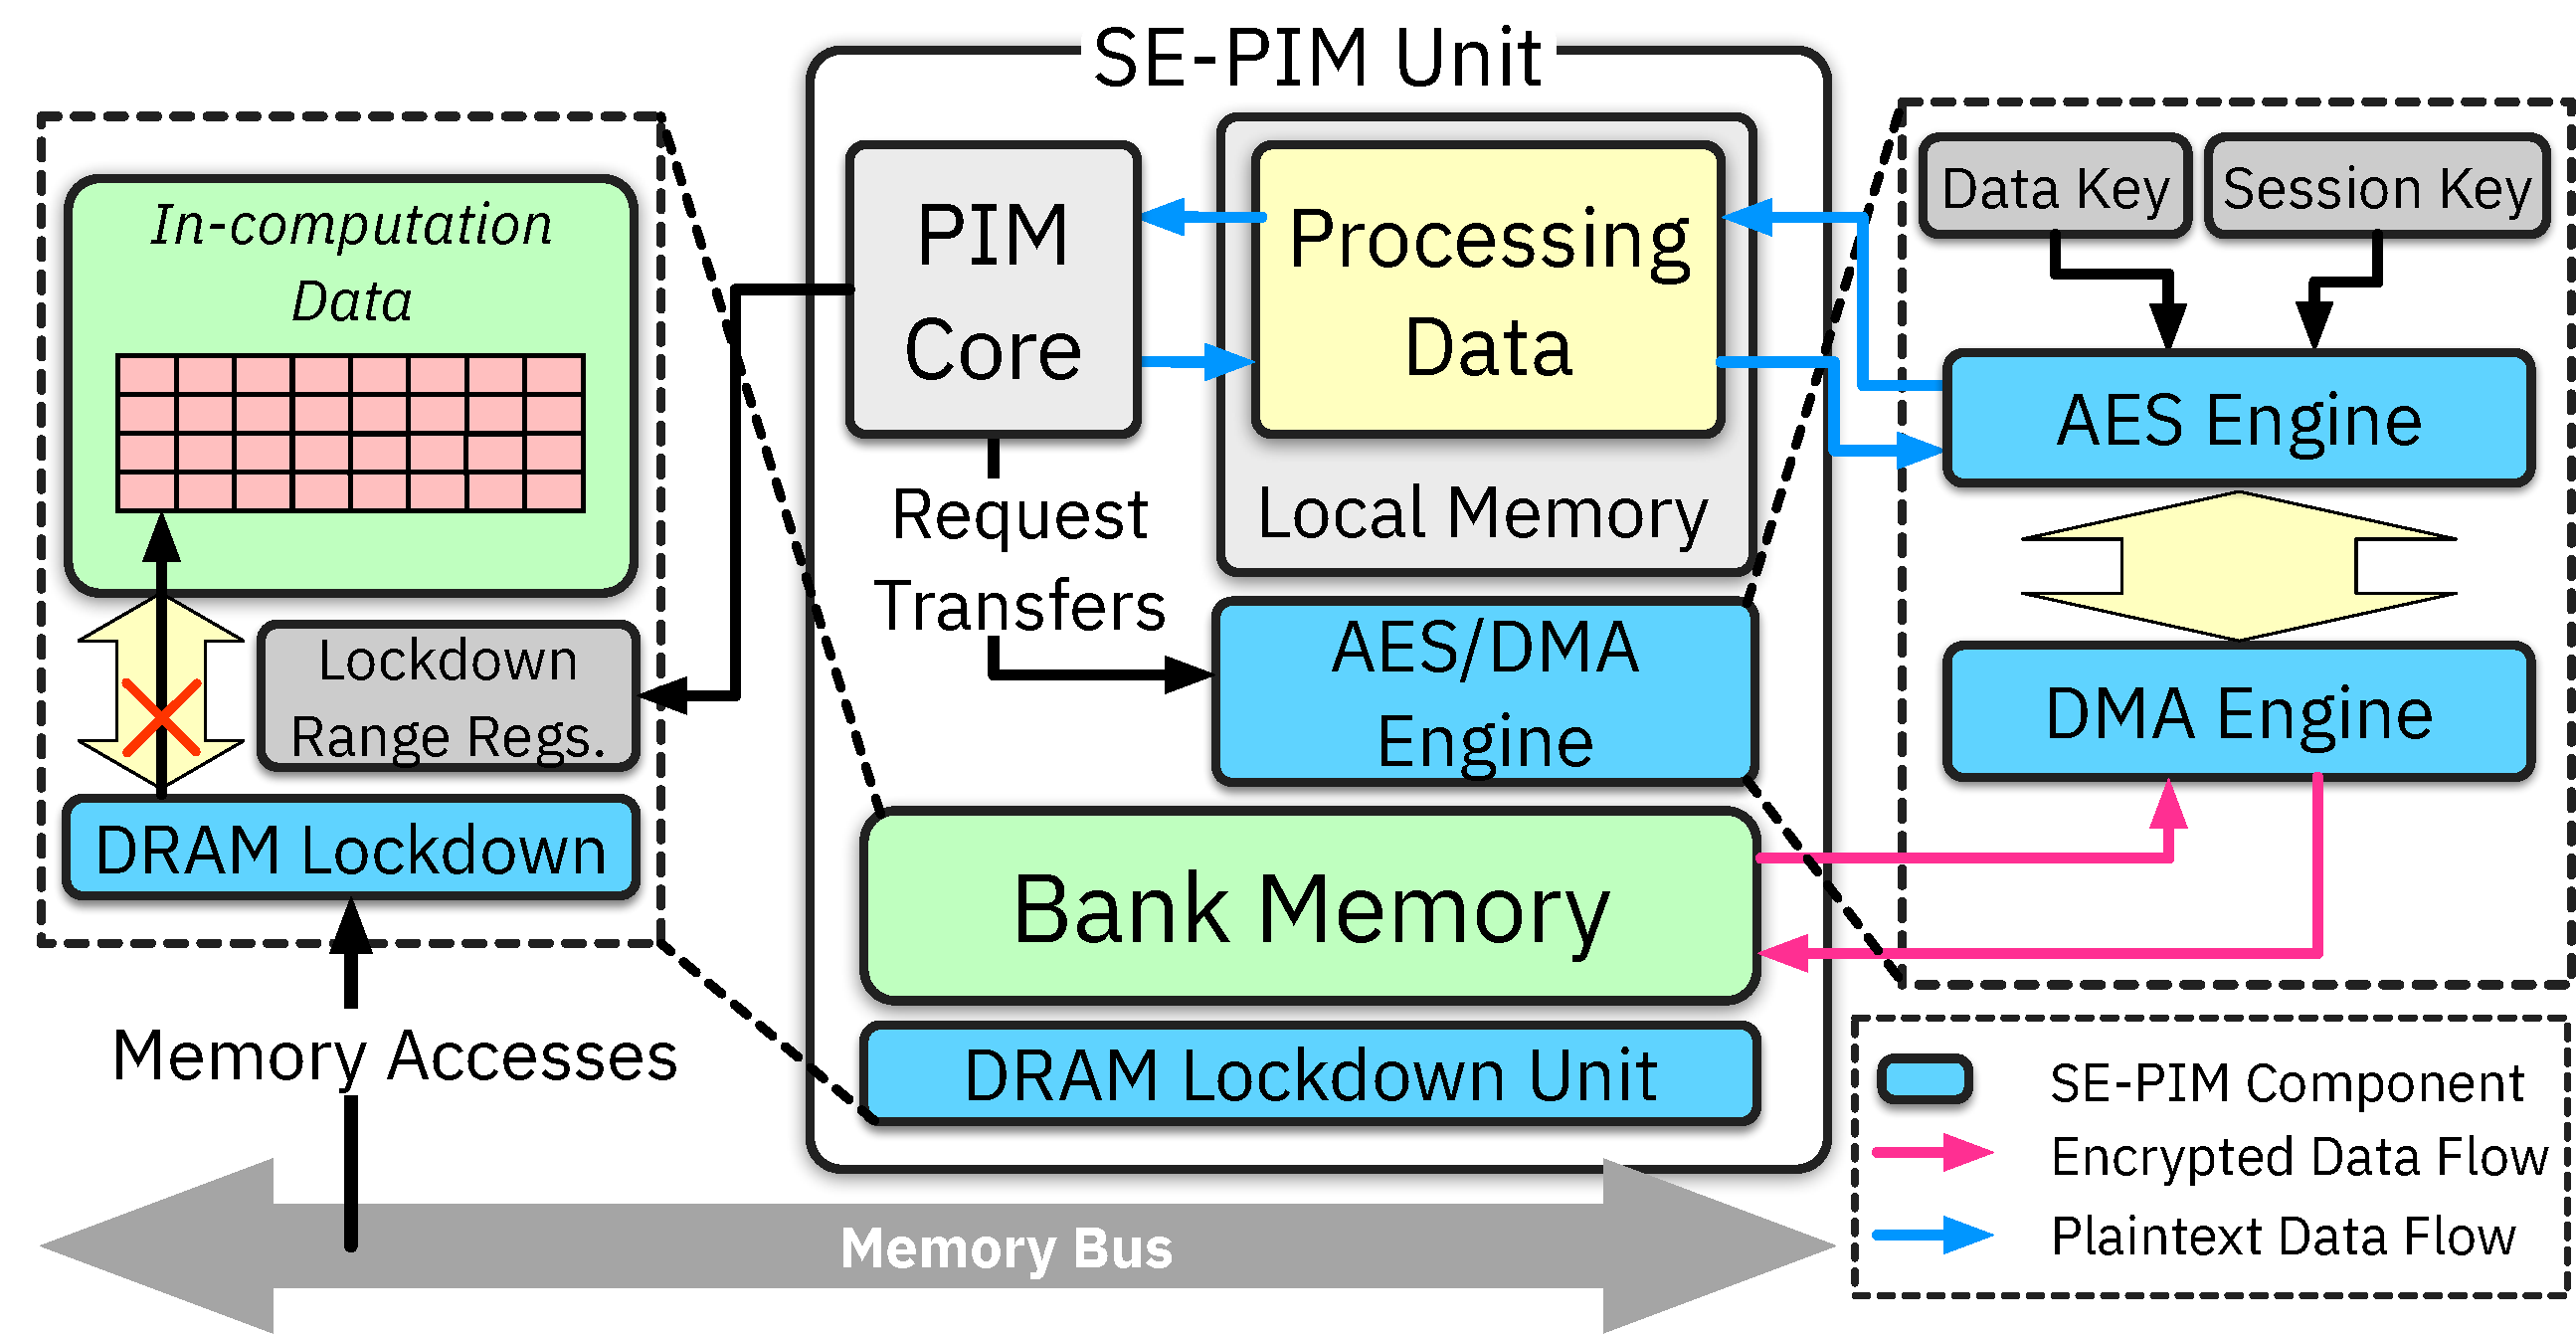
\includegraphics[width=.90\columnwidth]{figures/sepim/components.pdf}
    \caption{Overview of \thename hardware architecture.} 
    \label{fig:overview}
\end{figure}

\subsection{Overview}
\label{subsec:hardware}

% Internal
\autoref{fig:overview} shows the \thename architecture. \thename hardware design contains modifications to the \baseline architecture mentioned in \cref{subsec:pim-baseline} to protect the confidentiality and integrity of in-memory computations.
In \thename, the memory banks serve as a conventional main memory for the host and storage for encrypted data during confidential computing. A \emph{\thename unit} is included in each memory bank. Each \thename unit is equipped with a PIM core, PIM local memory, \emph{DMA/AES engine} and \emph{DRAM lockdown unit}. The functions of the PIM core and local memory are similar to that of \baseline. The AES/DMA engine introduces hardware acceleration to the DMA engine that significantly accelerates encrypted data transfers. The DRAM lockdown unit enforces \emph{DRAM lockdown}, a mechanism that prevents unauthorized access into the protected data during confidential computation. The DMA/AES engine and DRAM lockdown unit are hardware modules controlled by the PIM core running \thename kernel through MMIO registers. ROM and key storage are also introduced that can be used by all \thename units within a memory module. ROM includes cryptographic primitives (e.g., key pair generation, key signing) and preprogrammed procedures (e.g., attestation) that serve the \emph{commands}. The key storage contains the root endorsement key (EK), the root of trust to enable remote attestation. 

%The host enclave communicates with \thename through two interfaces, an in-memory DMA buffer and MMIO registers. 

We will further elaborate how a host enclave uses \thename through our programming model in \cref{sec:prog-model}. \emph{\thename components} in \autoref{fig:overview} (DMA/AES engine, DRAM lockdown unit) are the new hardware components that we introduce to enable confidential computing acceleration. We will explain the necessity and functionalities of the remaining components in the following subsections. 
 

\subsection{Remote Attestation and Secure Communication Channel} 
\label{subsec:attestation}
\label{subsec:communication}
\label{subsec:secure-channel}


To enable attestation and secure channel establishment, we introduce a ROM containing the code for attestation and key exchange and key storage with the root endorsement key (EK), which functions as the root of trust.
% \hdr{Key exchange.}
% Why attestation
% The capabilities for remote attestation and secure session establishment are the minimum requirements for \thename to be a trusted storage device (\goal{1}). In \thename, the components that enable these functionalities are the ROM and the key storage.
% The attestation process between a processor enclave (i.e., SGX) and an external entity (e.g., a secure accelerator) is well-documented and provided with an ample amount of examples~\cite{sgx-ra,sgx-ra-tls,graviton,invisimem,trustore,sdimm}. We apply the same principles employed in the previous works to enable remote attestation and key exchange. In particular, 

\hdr{Remote attestation. } 
Remote attestation allows a remote challenger (e.g., the CPU-side enclave) to verify the authenticity of the hardware by verifying \thename's certificate with a certificate authority (CA). The host enclave first obtains the \thename unit's certificate with the command \texttt{GET\_CERT}. The unit first generates an attestation public/private key pair from the EK inside the key storage. It signs the public attestation key with the endorsement key and then writes it to a memory buffer accessible by the enclave. The enclave then verifies the certificate with the CA of \thename (e.g., the manufacturer of \thename). The public key is extracted from a verified certificate and used for key exchange. 


\hdr{Secure communication channel establishment.} 
After remote attestation, the host enclave creates and shares a symmetric session key with a \thename unit to establish an encrypted channel for sending commands and parameters. The session key is encrypted with the public attestation key and sent to \thename as the argument to the command \texttt{SET\_SESSION\_KEY}. The session is used to encrypt all parameters sent to the parameter channel. We will further describe how the channel is initialized and used in \cref{sec:prog-model}. The host also shares a \emph{data encryption key} with \thename using the command \texttt{SET\_DATA\_KEY}. The data encryption key is used to encrypt and decrypt data stored in memory to be processed by \thename.  
%\hdr{Secure communication channel.}
We use authenticated encryption, e.g., AES-GCM, to provide authenticity and integrity to the communication channel. A monotonically increasing counter is also used to achieve resistance against replaying. Moreover, we employ fixed communication messages on the channel to prevent side channels.

\hdr{Commands authorization.} 
The use of authenticated encryption on the parameter channel also prevents unauthorized entities from issuing commands to \thename. When a command does not require parameters (e.g., \texttt{LOCK\_MEM}) is used, the host enclave encrypts and sends a nonce to the parameter channel to be used by \thename to authenticate the sender of the command. The \texttt{GET\_CERT} and \texttt{DESTROY} commands (described in \autoref{tab:commands}) do not require authentication. \texttt{GET\_CERT} is used before the secure communication channel is established. On the other hand, an unauthorized \texttt{DESTROY} command counts as a denial-of-service and does not compromise the integrity and confidentiality of \thename's execution.

%Similar to other proposals for hardware accelerator attestation~\cite{graviton,invisimem,sdimm}, our attestation protocol only attests \thename to the processor enclaves using them. Mutual attestation (e.g., to only allow authorized developers to load programs on a \thename unit) is also possible, following the secure boot process of FPGA devices~\cite{trustore}. 

% We implement the following commands for the attestation and key exchange process: \texttt{GET\_CERT} and \texttt{SET\_SESSION\_KEY} (\autoref{tab:commands}). 
% What is different/mutual attestation

%Furthermore, it is crucial to prevent a \thename unit from leaking the EK since it is the root of trust for \thename. First, we only allow the attestation procedure to access the EK. As noted by \cite{minimalist}, the requirement can be easily enforced with the introduction of a hardware monitor on a PIM core’s program counter that only allows access to the EK when the counter is within the attestation code (inside ROM). Moreover, for each newly created \pimenclave, new public and private key pairs used for attestation are derived from the EK to prevent information leakage about the EK. 

% On receiving the key, \thename writes the key into the AES engine and uses it to encrypt/decrypt the following communication messages on the parameter channel.

% %\hdr{Session key and data key.} 
% In addition to the secret session key, which is used for the DMA-based secure communication channel between \thename and the host, 
\subsection{Hardware Acceleration of Encrypted Data Flow }
\label{subsec:performance}
\label{subsec:aes-dma}
% \subsection{Software AES on Real PIM Hardware}
\label{subsec:upmem-aes}


% \autoref{fig:aes} describes the AES-capable DMA engine and its operation. 
Since \thename stores encrypted data inside the memory, encrypted data flow is fundamental to our computation model. However, the PIM core is a general-purposed processing core; it must operate on plaintext data. Hence, after loading them into local memory, data from the memory banks must be decrypted before processing. Furthermore, the \thename kernel might need to replace the old in-memory data block with new data after computation, which requires encryption before the transfer. As we explained in \cref{subsec:challenges}, software-based encrypted data movement between PIM and memory creates a substantial bottleneck in an evaluation on real PIM hardware. Hence, we deem the inclusion of AES acceleration essential for our system to function as an accelerator for large data computation.


\hdr{AES-enabled DMA engine.} We propose the use of an AES-acceleration-capable DMA engine. An ISA extension for AES acceleration (e.g., x86 \texttt{AES-NI)} can improve the encrypted data transfer performance. However, we argue that it would consume a significant portion of the PIM core cycles that could have been used for data computation. Also, such a requirement creates an unnecessary constraint in the PIM core design, which is commonly limited in processing power~\cite{upmem-atc}. On the other hand, implementations of AES-enabled DMA engines already exists~\cite{nxp,advanced-dma-controller} and can be easily incorporated into existing hardware due to its predictable power and area requirements. The introduction of such an acceleration engine can be an indispensable component in achieving confidential data-intensive computing. 

We design the AES-enabled DMA engine as a hardware module integrated with the PIM core through MMIO. The PIM core configures the hardware with the keys (\texttt{SESSION\_KEY} and \texttt{DATA\_KEY}) exchanged during secure channel establishment with the host enclave. After, all data transfers between the bank and PIM local memory by the DMA engine are simultaneously encrypted/decrypted using the shared keys. Data would arrive decrypted at the PIM local memory from the memory bank and vice versa. We further explain the details of the component and our simulation methodology in \cref{subsec:impl-aes}.


\subsection{Preventing Side-channels and Tampering During Computation}
\label{subsec:side-channels}
% We demonstrate in \cref{subsec:challenges} that there are attack vectors on \baseline that compromises the confidentiality and integrity of the protected computation. 

% We demonstrate in \cref{subsec:challenges} that there are attack vectors on \baseline that compromises the confidentiality and integrity of the protected computation. 
In this section, we elaborate on the components and their functionality that help us overcome the challenges outlined in \cref{subsec:challenges} (\challenge{2}, \challenge{3} and \challenge{4}). We introduce two techniques to \baseline, \emph{DRAM lockdown} and \emph{controlled memory access channel}. DRAM lockdown allows the host enclave to disable host-side accesses into the memory region containing data, thus hiding the memory content changes leaked by the \thename kernel's computation. We also eliminate the splicing and replaying attacks by preventing unauthorized memory writes. Our controlled memory access channel provides an interface for the host enclave to perform memory accesses without leaking the address side-channels. It accepts encrypted memory requests through the parameter channel and let \thename performs the actual memory operation on behalf of the host enclave. The channel hides access pattern leakages on the memory bus when DRAM lockdown is active. We now go over the detailed description of each technique.

%\subsection{DRAM Access Control}
\subsubsection{DRAM Lockdown}
% \hjc{memory access control may be confusing, DRAM lockdown?}


\label{subsec:access-control}
\label{subsec:selective}
Our DRAM lockdown mechanism efficiently addresses both \challenge{3} and \challenge{4}. The design of DRAM lockdown is based on the following observations about PIM computation. First, applying the ORAM algorithm (described in \cref{subsec:oram}) to hide the memory access pattern of \thename kernels would incur significant performance degradation and complexity to our design~\cite{zerotrace,freecursive-oram}. Ultimately, the use of ORAM would make \thename unusable as an accelerator for large data computation. Second, we observe that memory integrity can also be provided when only authorized accesses can update the memory. An alternative approach is to introduce a memory verification engine that performs a check for each encrypted data block by comparing a block's counter value with the protected value~\cite{bonsaimerkletree,common-counter}. However, the introduction of such a memory verification engine does not address \challenge{3} and would inadvertently introduce extra overheads for memory accesses~\cite{bonsaimerkletree,common-counter}.
Finally, we observe that most data movements occur at the start of the PIM workload, where the host loads data into the memory bank. After the initial data transfer, the data rarely leaves the memory banks and is commonly reused in place by the PIM core. The host enclave can also offload different kernels to process the same data within memory. Hence, the direct access into memory from the host side can be safely disabled during PIM computation. 

% On the other hand, a memory verification engine, such as the ones proposed in \cite{bonsaimerkletree} and \cite{common-counter}, would provide the memory protection against slicing and replaying.

% %First, even with the introduction of a memory integrity checking engine, 
% Based on the observation, denying the host access to memory is also the most efficient approach to solve. 
Based on the observations above, we conclude that denying host access to the memory regions containing data for \thename computation is essential to eliminate the memory content change side-channel (\challenge{3}) while also providing protection against splicing and replaying (\challenge{4}).
We observe that the placement of data into the memory banks only leaves a \emph{sequential} pattern with very little information to be leaked. This is because the memory side-channels happen \emph{during} calculation due to a distinct pattern of behavior in the code~\cite{raccoon,sgx-cache-attack,membuster}. Hence, we allow the usage of direct memory mappings to load data into the memory banks efficiently. After data have been located inside memory, the host enclave can request a \emph{lockdown} of memory by sending a \texttt{LOCK\_MEM} command to the \thename unit. \thename, in turn, configures the lockdown range registers in DRAM lockdown unit only to allow access to the DMA-based secure communication channel, which is protected by authenticated encryption. We describe the implementation of this mechanism in \cref{sec:implementation}. To remain functional as memory storage during bank lockdown, we provide a data channel that allows the host to send encrypted memory requests to \thename, which we describe in \cref{subsec:secure-access}.


%However, we allow the host enclave to make efficient data transfers using direct memory mappings, as t
% host-side direct accesses to the memory can be safely disabled during \thename computation to turn the \thename banks into protected memory regions.

%In \thename, we introduce an \emph{access control unit} that enforces \emph{selective memory access control} on every host-side incoming memory request on the memory bus. 
% 1. Direct Write 2. Lock 
% 1. DMA the data  2. Lock 3. Measurement


\hdr{Bank memory integrity measurement.} Even with the lockdown mechanism, the attacker could still perform tampering attacks (e.g., splicing and replaying) in the time window between the data load and DRAM lockdown. We implement a memory integrity measurement to thwart such attacks. Upon receiving the \texttt{LOCK\_MEM} command, \thename takes the measurement of the data received and sends it to the host enclave. The host enclave compares the measurement to the precomputed hash value of the data to confirm that it has not been tampered with. Measurement must be performed every time the memory bank is unlocked for data transfer, then locked to guarantee memory integrity. 



\subsubsection{Controlled Memory Access Channel} 
\label{subsec:secure-access}
% \kha{rewriting}
We introduce a channel for the host enclave to access the memory bank \emph{during} DRAM lockdown, called the \emph{controlled memory access channel}. The channel provides exclusive access to only the authenticated entities (i.e., the host enclave) while the DRAM lockdown is in effect. The channel adopts a similar approach to the related works that build a secure communication channel between the secure enclave and memory~\cite{trustore,invisimem,obfusmem}. The essence of channel is that \emph{access addresses} and the \emph{operation} of the memory request is encrypted as parameters of the new data access commands, while the actual data access is offloaded to \thename. Since the DRAM lockdown mechanism already protects the access pattern of \thename, memory accesses from the host enclave performed through this interface are also resistant against the \emph{address side-channel} on the memory bus (\challenge{2}). For this channel, we implement the \texttt{ACCESS\_DATA} and \texttt{MEMCPY} commands for the host enclave to securely perform data access and movement~(\autoref{tab:commands}).

%encrypted memory request as the \emph{parameters} for the \texttt{ACCESS\_DATA} and \texttt{MEMCPY} commands (\autoref{tab:commands}). 

\begin{figure}[t]
    \centering
    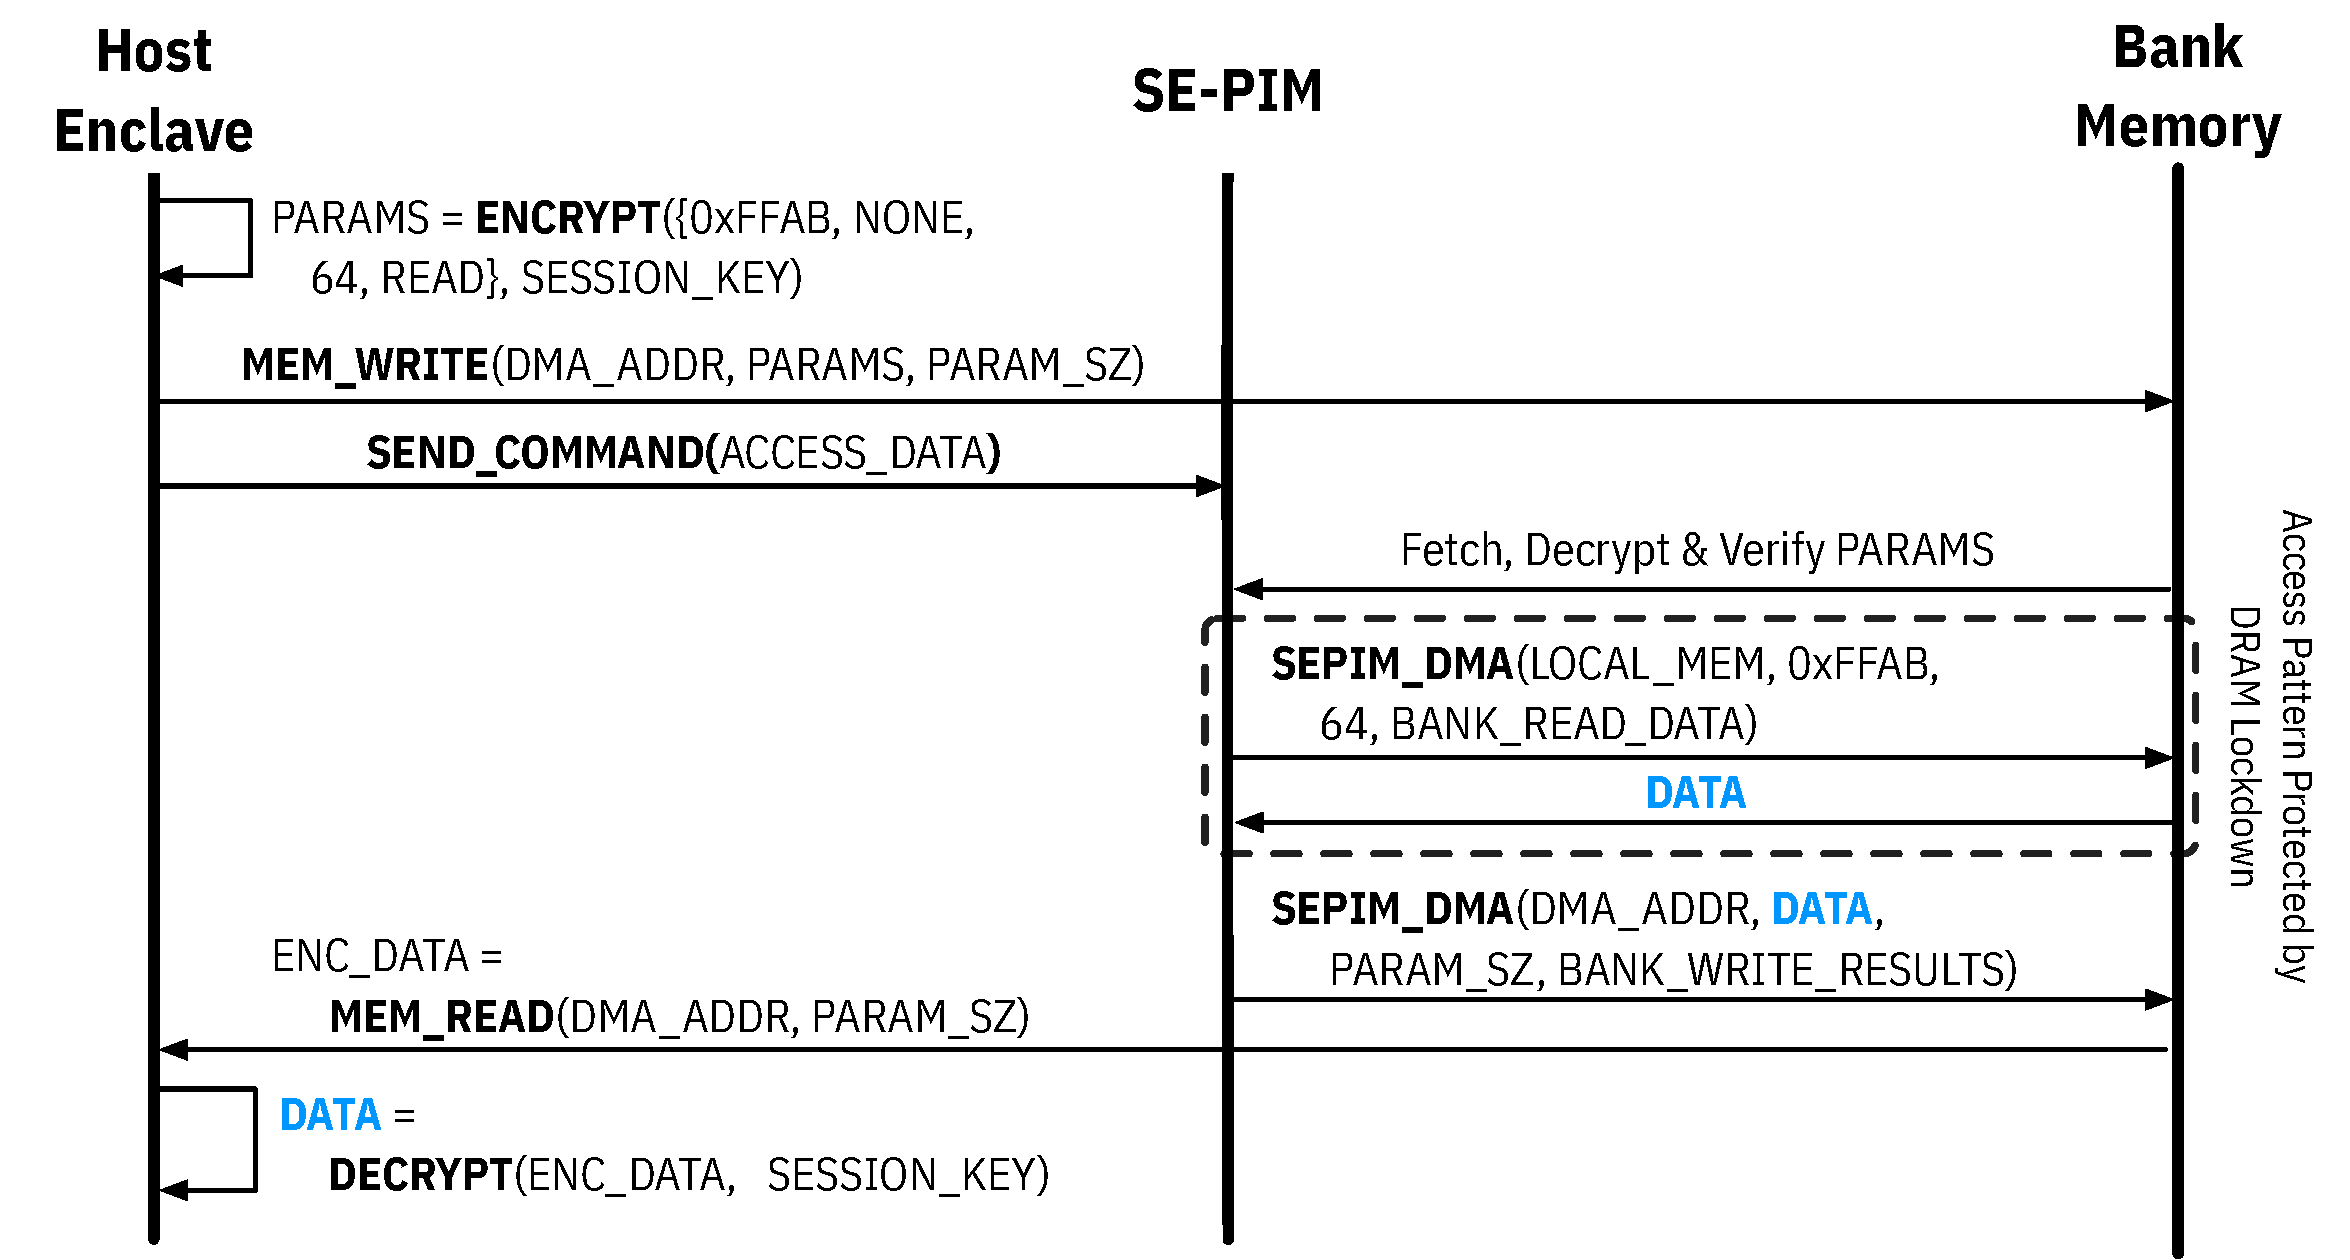
\includegraphics[width=0.90\columnwidth ]{figures/sepim/secure_access.pdf}
    \caption{An example of data read using controlled memory access channel. The data access pattern of host is protected by encryption, while the data access pattern of PIM kernel is protected by DRAM lockdown.}
    \label{fig:secure-access}
\end{figure}

\hdr{Controlled data access.} \texttt{ACCESS\_DATA} allows the host enclave to read or write a block of data during bank lockdown while hiding the access pattern from observers. Parameters for \texttt{ACCESS\_DATA} are the encrypted data block, the requested address, the size of access, and the type of operation (read or write). Instead of introducing separated commands for data read and write, we define the type of access in the parameters to mimic the security guarantees of oblivious RAM algorithms~\cite{path-oram}. \autoref{fig:secure-access} shows the data access from the host enclave using \texttt{ACCESS\_DATA}. First, the encrypted parameters are written into the DMA-based secure channel, and the command is sent to the \thename unit. The \thename unit will decrypt and fetch the memory request into its local memory on receiving the commands. The data block is placed in the requested location for a write request. Otherwise, on reading requests, the \thename unit fetches the block, encrypts, and writes it to the secure channel. Collaboration from the host enclave is required to achieve full ORAM-like security properties. Namely, to hide the type of memory access, the memory requests must contain dummy data on a read, and a dummy read request must follow every write request.

\hdr{Controlled data movement.} The \texttt{MEMCPY} command instructs \thename to copy data from one address to another, which is useful when data is already located inside the memory. On receiving the command, \thename will fetch the requested data block to local memory and write it to the destination address. The operation performs data movement using the fast internal bus on PIM, which reduces expensive data transfers on the memory bus.

% \hdr{Controlled data movement.} 




